\documentclass[titlepage]{article}

\usepackage{color}
\usepackage{courier}
\usepackage{graphicx}
\usepackage{hyperref}
\usepackage{indentfirst}
\usepackage{lipsum}
\usepackage{listings}
\usepackage{textcomp}
\usepackage{todonotes}
\usepackage{xcolor}

\lstset{basicstyle=\footnotesize\ttfamily,breaklines=true,language=SQL}
\lstset{framextopmargin=0pt,frame=single}

\lstdefinelanguage{ProtoSQL}%
{%
	otherkeywords={ProtoSQL>,?,->,=>,x>,\{,\},//,\\\\,null}%
}

\lstdefinelanguage{EBNF}%
{%
	language=XML,%
	otherkeywords={?,+,*}%
}

\newcommand{\FS}{\textit{F\nolinebreak\hspace{-.05em}\raisebox{.5ex}{\small\bf \#}}} % http://www.johndcook.com/blog/2011/10/18/typesetting-c-in-latex/

\begin{document}

	\thispagestyle{empty}
	\topskip0pt
	\vspace*{\fill}
		~\centerline{\textcolor{red}{\Huge{WORK IN PROGRESS}}}
		\newline\newline

		\large{Known Issues}
		\begin{itemize}
			\item Adobe renders the 2.2 (The Parser) AST images oddly unless zoomed in.
			\item Fix code examples so it's still centered but left aligned.
		\end{itemize}

		\listoftodos
	\vspace*{\fill}

	\newpage

	\thispagestyle{empty}
	\title{Exploring Best Practices for the Creation of a Programming Language Compilation System: A Case Study with ProtoSQL}
	\author{Brandon Browning}
	\maketitle

	\begin{abstract}
		Developing a programming language is a process full of managing many different forms of complexity.  This project is an experiment in managing the problems that may arise in the development of a compilation system for a new programming language; it is meant to explore and evaluate the best practices through the creation of a full language.  This will result in an industrial-strength and full-featured tool chain, including a parser, optimizer, and compiler.  The parser will adhere to the language grammar, generate descriptive error messages, and supply an Abstract Syntax Tree (AST) to the optimizer.  The optimizer will then go through the tree and rewrite pieces as it sees fit, generally to improve performance.  Then the compiler, here a cross-compiler, will take the AST and output corresponding SQL code.

	\end{abstract}

	\newpage

	\thispagestyle{empty}
	\tableofcontents
	\listoffigures

	\newpage

	\setcounter{page}{1}

	\section{Insight}

		This project started out with a deep curiosity into how languages are defined, and how people manage the tooling around them.  To someone who is unfamiliar with workings of parsers and compilers, it seems like such an immense and magical process to have code that turns code into code.  It's always a bit magical, but I hope through this paper to show how the field of Computer Science has dealt with this problem, and why it's not as painful as one would think.

		First I'll go over some of the ideas behind programming languages; such as why new ones should be created, the ecosystem surrounding them, and how different ways they're implemented.  Then I'll describe the process behind the creation of ProtoSQL; including the difficulties faced, the benefits of some of the practices employed, and the overall experience and outcome of working on a new programming language.

	\section{Overview of Creating a New Language}

		Languages are usually created because there's some kind of problem one would like to solve; such as wanting to work at an abstraction level between two other languages, or a completely different way of thinking to some established standard.  Over time, the strengths and weaknesses of a language begin to show.  The weaknesses are not necessarily oversights by the original designer, but more intricacies that are brought out over time by heavy usage of the language.  Due to this phenomenon, the development of new languages serves an important role in the evolution of software.

		\subsection{The Grammar}

			The first part of the process towards the foundation of a new programming language, almost out of necessity, is to develop the syntax and semantics of how the language will function.  There's an already existing domain of problems that the creator wants to solve, so they must think on the constructs used to solve that problem, and how they will fit together.  For example, if someone wanted to create a language for a hand-held algebra system, they'd have to consider brevity and ease of entry as design goals.  They may opt to limit the feature set and complexity of the language as it's probably aimed at beginners, and the limited input versus a desktop-based system would be a significant factor.  At this point, many of the details aren't known, but the high-level design starts coming in to play which heavily dictates the initial direction of the language.

		\subsection{The Parser}

			Usually the first part of a new programming language compilation system to be implemented is the parser.  The construction of a parser helps solidify the correctness of the grammar, lets you start working on and provides a basis for the compiler, and helps iron out and explore the grammar.  If the language hasn't been carefully scoured over before work on the parser begins, then problems in the grammar naturally surface during work on the parser.

			Now what exactly does the parser do?  The parser is the engine that turns the source text, or the source material for the entire process, into a structure fed through the rest of the system until completion; this structure is known as an Abstract Syntax Tree (AST).  The AST is a representation of the grammar in the form of a manipulatable data structure.  The primary purpose of the parser is then to turn the source text into its corresponding AST.

			The AST could be visualized as a tree or graph data structure which is common in Computer Science, and where the name comes from; however, this is beyond the scope of the paper.  Essentially, it is a hierarchal structure of the pieces of the language that the source text demonstrates.  For example, here's a simple arithmetic expression:
			\newline

			~\centerline{\Large{$x + 5$}}
			\newline

			This could be represented graphically, slightly simplified, as Figure 1
			\footnote{AST Graphics generated from \href{http://www.gliffy.com}{gliffy.com} and manipulated with \href{http://www.getpaint.net/}{Paint.NET}}.
			\newline

			\begin{figure}
				\caption{Simple Addition AST}
				~\centerline{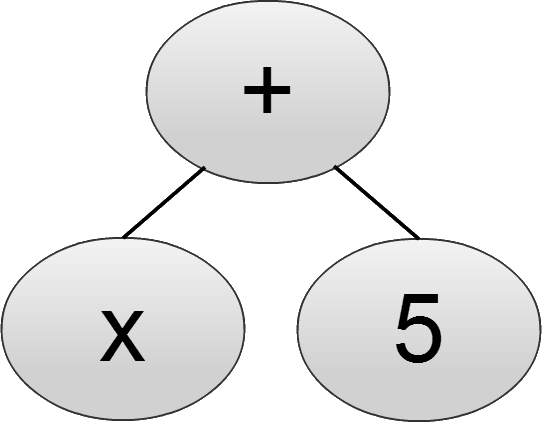
\includegraphics[scale=.3]{ExampleSimpleAST.png}}
			\end{figure}

			\newpage
			A more complex programming-language type expression might be:
			\newline

			~\centerline{\Large{$printf(''(\%d, \%d)'', x, \frac{1}{2})$}}
			\newline

			An AST that's much more similar to how the above expression would be treated in an industrial-strength parser is shown in Figure 2.
			\newline
			
			\begin{figure}
				\caption{Complex AST}
				~\centerline{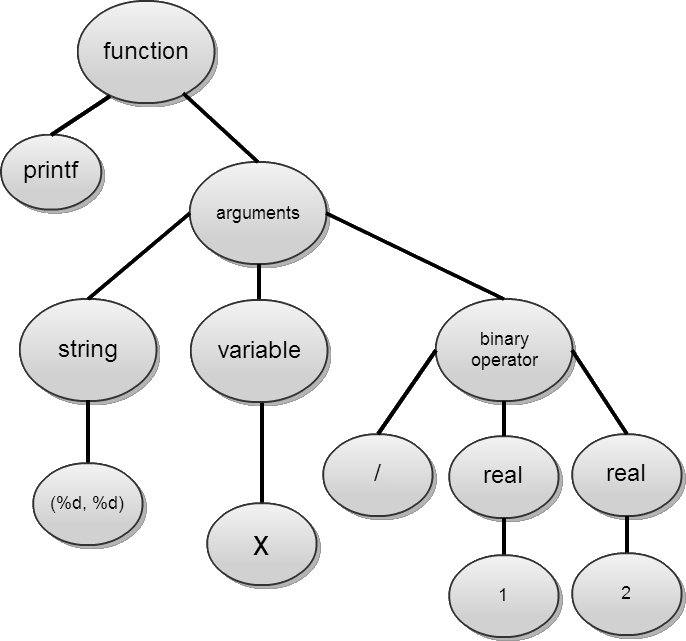
\includegraphics[scale=.5]{ExampleCodeAST.png}}
			\end{figure}

			Here, many of the important details left out of the previous graphic are shown.  The above AST does not have any information as to what plus, x, and 5 are.  Here, we see that at the highest level is a function being called, named printf, which has three arguments.  The type of the argument, as well as its value, are recorded.  Having the tree structure this way makes it quite easy to make optimizations.

			There are two main types of parser implementations; parser generators and less common parser combinators.  Parser generators convert a description of the grammar in a special format, mixed in with pieces of logic, into a new program which parses that grammar.  Parser generators are some of the first parsers made, and produce quite efficient code; however, there is an extra layer of indirection in producing the parser, and the input source code is generally a superset of the language the logic is written in.

			On the other hand, parser combinators are less often used, partially to being relatively new.  They contrast from parser generators by just being a library used to write your parser, not a proprietary extension, and there is no extra step of generating the parser; the code \textit{is} the parser.  Parser combinators work differently from parser generators by building up large parsers from little parsers.  For example, one may create the functionality to turn any parser into a new parser that parses a comma-separated list of the original parser.  Suppose our original parser is one that parses integers, such as:
			\newline

			~\centerline{$-42.3$}
			\newline

			Applying our comma-separated list parser combinator to our integer parser will parse:
			\newline

			~\centerline{$-1, 13, 15.6, -.1$}
			\newline

			Then, given another function that parses the input parser surrounded by square brackets, you could generate a new parser resembling:
			\newline

			~\centerline{bracket(comma-seperated(bracket(comma-seperated(parse-number))))}
			\newline

			Which could parse the following:
			\newline

			~\centerline{$[[1, 2], [-1, 42.5], [1]]$}
			\newline

			Creating this parser took almost no effort, and as a bonus, all of the intermediate parsers are available to us.  This way, building up a parser for your grammar allows you to, for free, get all of the parsers you create on the way.  Everything is defined in a composable way, and it's exciting to put together mini-parsers to create a large system.

		\subsection{The Optimizer}

			Optimizers exist to improve the performance of the output.  Generally, a programming language is devised to address difficulties in other languages, and also to provide abstraction; optimizers are an important part in both roles; they can be smarter than previous languages, allowing some of the pains previously endured creating the old language's programs to disappear, and also to allow new abstractions to not come at a high cost.

			The optimizer would be a tool that transformers the AST generated by a parser into a more performant, similar AST, that should effectively behave exactly the same.  For example, the optimizer may crawl down the tree and find the addition operator being used on two constants:
			\newline

			~\centerline{$delay = duration() * 60 * 1000$}
			\newline

			Here, it may optimize away the multiplication and replace it with the only possible result, which is known as inlining.  The new source may then have this line instead:
			\newline

			~\centerline{$delay = duration() * 60000$}
			\newline

			This is obviously quite a simple optimization, but it's easy to show and understand how the behavior of the program shouldn't differ from the previous version.  Optimizations like this, but much more complex, can a significant amount of a program's execution time.

		\subsection{The Compiler}

			The role of the compiler is to translate the optimized AST into the target code.  The target of a compiler is usually another language, whether it be one of the same abstraction level, or something much more low-level.  It does this by going through the AST, and deciding how it should output.  Usually this is a recursive process, which when completed leads the the final output and end goal of the programming language; to end up in some other form.  Note the entire process from parsing through compilation is sometimes just known as compiling.

			For example, there may be a compilation system for converting an arithmetic expression from infix to postfix.  This problem could be solved by defining a grammar for infix arithmetic, then parsing it into an AST, and then traversing it in a way that will put the operations in post order.  Given an expression, such as:
			\newline

			~\centerline{\Large{$1 + \frac{5}{3}$}}
			\newline

			This could be represented as the AST in figure 3.
			\newline

			\begin{figure}
				\caption{Post Order AST Example}
				~\centerline{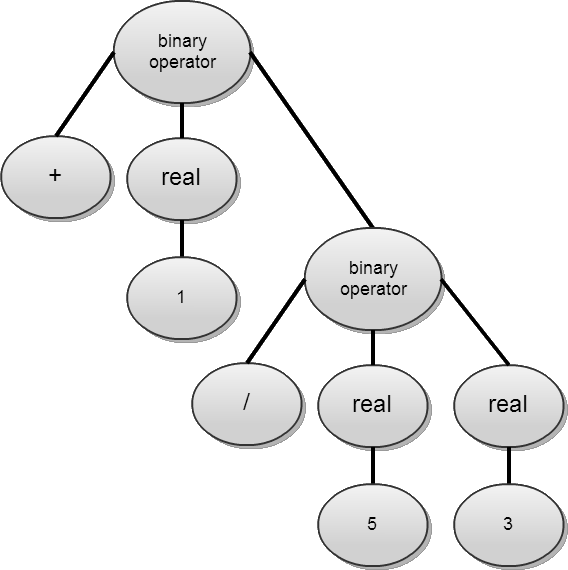
\includegraphics[scale=.5]{ExampleCompileBinaryAST.png}}
			\end{figure}

			The compiler could then recursively traverse down the tree.  If it encounters a real number, it outputs it.  If it encounters a binary operator, however, it will recursively output its children, and then the operator name.  A listing of how this process would occur is shown in Figure 4.
			\newline

			\begin{figure}
				\caption{Post-Order Steps}
				\begin{enumerate}
					\itemsep0em
					\item $compile(1 + \frac{5}{3})$
					\item $compile(1)\ compile(\frac{5}{3})\ +$
					\item $1\ (compile(5)\ compile(3)\ /)\ +$
					\item $1\ 5\ 3\ /\ +$
					\newline
				\end{enumerate}
			\end{figure}

	\section{Implementation of ProtoSQL}

		ProtoSQL began as a combination of two things; a curiosity into the inner-workings of programming languages, and a desire to find an alternative to SQL (a database manipulation language).  Programming languages are an extremely important part of the software ecosystem, and I wanted to explore the way they transform text, make smart decisions, and translate it into another domain.  My desire to explore alternatives to SQL comes from a productivity point-of-view, not necessarily from a disagreement with its design; SQL is an old language, and I thought there would be some ways to make development with it less painful.  It does, however, do its job very well; it just is quite unwieldy and verbose.

		\subsection{The Grammar}

			My main design goal was a succinct grammar that captured the common use-cases for SQL.  I was mostly targeting the exploratory SQL code written to hunt down problems, the ad-hoc queries that aren't generally kept around.  I felt this subset of SQL code was an important target as it always seemed to take excessive time, and it seemed there could be a better system.

			I began work on a grammar that stayed consistent throughout the process.  There were a few changes, however they were mostly things that were unimportant in the scheme of things, such as what characters separate different constructs.  Some early pieces of ProtoSQL that worked successfully are shown in figure 5.
			\newline

\begin{figure}
	\caption{Early ProtoSQL Queries}
	\begin{lstlisting}[language=ProtoSQL]
> SomeTable
	\end{lstlisting}

	\begin{lstlisting}[language=SQL]
SELECT *
FROM SomeTable;
	\end{lstlisting}

	\begin{lstlisting}[language=ProtoSQL]
> SomeTable?id=5
	\end{lstlisting}

	\begin{lstlisting}[language=SQL]
SELECT *
FROM SomeTable
WHERE id = 5;
	\end{lstlisting}

	Note: The ProtoSQL code will come after a caret (\textgreater) and a space; however, this is not necessary in the language itself; it is only done here to differentiate from the following SQL.
\end{figure}

		\subsection{The Parser}

			The parser was the part I was most looking forward to, and in the end the part I thought was most interesting and exciting.  One of my side goals in this project was to work on the \FS programming language, so I chose the parser combinator library FParsec\footnote{Available at \url{http://www.quanttec.com/fparsec/}}, to provide the parsing primitives I'd use to build up my ProtoSQL parser.  This is essentially the standard parsing library for \FS, and it also seemed extremely interesting.

			Creating the initial low-feature parser was exciting.  First I toyed around with the library testing how the different tools work, even creating a miniature yet functional JSON\footnote{According to \url{http://www.json.org/}, `JSON (JavaScript Object Notation) is a lightweight data-interchange format'} parser as a test.  Then I began working on the ProtoSQL parser.  Given my lack of experience with FParsec, I still made a usable parser quickly for the initial grammar.  I used this advantage and ease of parser implementation to essentially experiment with my grammar; a luxury I feel may not always arise with other tool-chains.

			As I began working on the compiler, I encountered issues with my parser; however, in the end it was always a case of trying to correctly express my grammar.  For example, with the following piece of code:
			\newline

			\begin{lstlisting}[language=ProtoSQL]
				> SomeTable?x=5/y
			\end{lstlisting}

			There was an ambiguous case that I did not consider.  I didn't expect the forward slash to act as division, but instead be an \textit{order-by clause}.  There is no ambiguity in a grammar, since the order that the definitions are written is significant, so the parser logically went with the case that I told it to use, which was in this case, division.  I felt if this could be confusing to users that I should use a different sign for the separator for an \textit{order-by clause}.  Hence, I changed it from \textit{/} to \textit{//}.  Therefore, the division case and then the \textit{order-by} case are respectively shown in Figure 6.
			\newline

			\begin{figure}
				\caption{Division / Order-By Problem}
				\begin{lstlisting}[language=ProtoSQL]
> SomeTable?x=5/y
				\end{lstlisting}

				\begin{lstlisting}[language=SQL]
SELECT *
FROM SomeTable
WHERE x = (5 / y);
				\end{lstlisting}

				\begin{lstlisting}[language=ProtoSQL]
> SomeTable?x=5//y
				\end{lstlisting}

				\begin{lstlisting}[language=SQL]
SELECT *
FROM SomeTable
WHERE x = 5
ORDER BY y ASC;
				\end{lstlisting}
			\end{figure}

		\subsection{The Optimizer}

			The optimizer for ProtoSQL is nonexistent.  SQL is a highly efficient language which optimizes itself.  As long as the database is configured well, the database does all the work to make queries efficient.  This is due to the fact in SQL you essentially say \textit{what} you want, not \textit{how} you want it.  This makes SQL quite difficult, and futile to optimize.  Therefore, instead of having an optimizer pass, the AST goes from the parser straight to the compiler.

		\subsection{The Compiler}

			To implement the compiler, I didn't use any other libraries or tools.  Essentially it involved smart work with text, and was more of a classical programming problem.  I had the least amount of problems working on the compiler, primarily due to the simplicity of SQL that I had to output.  Also, my AST format encodes all the information required, and the \FS language has many constructs making it easy to inspect the AST and generate the needed SQL code.  The style of my compiler essentially represents the one above in the overview.

	\section{Closing Thoughts}

		I thought this was an extremely exciting project, and am satisfied with the conclusion.  There's a unique feeling when I can enter any valid ProtoSQL code following my grammar, and it's magically transformed into the corresponding SQL I expect.  From here one could work on integrating the compilation system with an existing SQL tool, allowing you to essentially write ProtoSQL instead of SQL when doing ad-hoc database exploration and analysis.

		The code will be open-source and available under the MIT license, which allows it to be used for anything, but I am not liable for damages.  See the appendix for additional documents, including the grammar, code examples, and the MIT License.

	\section{Appendix}

		\subsection{Grammar Definition in EBNF}

\lstset{language=EBNF}
\begin{lstlisting}
; ProtoSQL - A succinct language that cross-compiles to SQL
;  for a Senior Honors Project
;  by Brandon Browning

; Assumed symbols:
;   <EOF>
;   <int>
;   <float>
;   <sql-string-text> ; For simplicity, the allowed SQL text between single quote (')'s in a string
;   <newline>
;   <tab>
; Note: No strings are escaped; instead the above symbols are used

<proto-sql> ::= 
	<data-expr> <spacing>
	<where-clause>? <spacing>
	<order-by-clause>? <spacing>
	<select-clause>? <spacing>

<data-expr> ::= <joins> | <table>
<joins> ::= <join> (<spacing> <join>)*
<join> ::= <table> <spacing> <join-arrow> <spacing> <table> <spacing> <join-tuple>?
<join-tuple> ::= "(" <spacing> <join-tuple-body> <spacing> ")"
<join-tuple-body> ::= <bracket-ident> (<spacing> "," <spacing> <bracket-ident>)?
<join-arrow> ::= "->" | "=>" | "+>"

<where-clause> ::= <where> (<spacing> <where>)*
<where> ::= "?" <spacing> (<where-id> | <value-expr>)
<where-id> ::= <tuple> | <int>

<order-by-clause> ::= <order-by> (<spacing> <order-by>)*
<order-by> ::= <order-by-type> <opt-spacing> <column>
<order-by-type> ::= "//" | "\\"

<select-clause> ::= "{" <spacing> <select-body> <spacing> "}"
<select-body> ::= (<select> <spacing> ";" <spacing>)* <select> <spacing> ";"?
<select> ::= (<ident-or-bracket> <spacing> "=" <spacing>) <value-expr>

<column> ::= <tri-string>
<table> ::= <tri-string>
<tri-string> ::= <ident-or-bracket> (<spacing> "." <spacing> <ident-or-bracket>){0,2}

<tuple> ::= "(" <tuple-body> ")"
<tuple-body> ::= <value-expr> (<spacing> "," <spacing> <value-expr>)* <spacing> ","?

<value-expr> ::= <binary-op> | <f-call> | <primative>
<primative> ::=  <string> | <int> | <float> | <literal>
<string> ::= "'" <sql-string-text>  "'"
<literal> ::= <ident>
<binary-op> ::= <value-expr> <opt-spacing> <binary-op-name> <opt-spacing> <value-expr>
<binary-op-name> ::= "&&" | "||" | "<" | "<=" | ">" | ">=" | "~" | "!~" | "=" | "!=" | "%" | "*" | "/" | "+" | "-"
<f-call> ::= <ident> <tuple>

<spacing> ::= <space-or-newline>?
<space-or-newline> ::= <space> | <newline>
<space> ::= " " | <tab>

<ident-or-bracket> ::= <bracket-ident> | <ident>

<bracket-ident> ::= "[" <bracket-ident-part>+ "]"
<bracket-ident-part> ::= <digit-letter> | <bracket-ident-symbol>
<bracket-ident-symbol> ::= <space> | "." | "/" | "\"

<ident> ::= <ident-head> <ident-tail>
<ident-head> ::= "_" | <letter>
<ident-tail> ::= "" | <digit-letter> <ident-tail>

<digit-letter> ::= <letter> | <digit>
<digit> ::= "0" | "1" | "2" | ... | "9"
<letter> ::= <lower-letter> | <upper-letter>
<lower-letter> ::= "a" | "b" | ... | "z"
<upper-letter> ::=  "A" | "B" | ... | "Z"
\end{lstlisting}

	\vspace{5mm}

		\subsection{ProtoSQL Code Examples}

\begin{lstlisting}[language=ProtoSQL]
ProtoSQL> Account ? FirstName ~= 'Jeff' && LastName != null
\end{lstlisting}

\begin{lstlisting}[language=SQL]
SELECT *
FROM Account
WHERE (FirstName LIKE 'Jeff') AND (LastName IS NOT NULL);
\end{lstlisting}

\begin{lstlisting}[language=ProtoSQL]
ProtoSQL> Purchase -> Account ? AccountType = 10 {
	AccountName;
	Total = Purchase.Amount
}
\end{lstlisting}

\begin{lstlisting}[language=SQL]
SELECT AccountName, Purchase.Quantity * Purchase.Price AS Total
FROM Purchase
INNER JOIN Account
    ON Account.AccountID = Purchase.AccountID
WHERE AccountType = 10;
\end{lstlisting}

\begin{lstlisting}[language=ProtoSQL]
ProtoSQL>
Account -> PurchaseAccount (AccountID)
PurchaseAccount -> Purchase
? AccountID = 42
? Purchase.Price > 0
{
	PurchaseID;
}
\end{lstlisting}

\begin{lstlisting}[language=SQL]
SELECT PurchaseID
FROM Account
INNER JOIN PurchaseAccount
    ON PurchaseAccount.AccountID = Account.AccountID
INNER JOIN Purchase
    ON Purchase.PurchaseID = PurchaseAccount.PurchaseID
WHERE AccountID = 42 AND (Purchase.Quantity * Purchase.Price) > 0;
\end{lstlisting}

		\subsection{The MIT License}

		Copyright (c) 2013 Brandon Browning
		\newline

		Permission is hereby granted, free of charge, to any person obtaining a copy of this software and associated documentation files (the `Software'), to deal in the Software without restriction, including without limitation the rights to use, copy, modify, merge, publish, distribute, sublicense, and/or sell copies of the Software, and to permit persons to whom the Software is furnished to do so, subject to the following conditions:
		\newline

		The above copyright notice and this permission notice shall be included in all copies or substantial portions of the Software.
		\newline

		THE SOFTWARE IS PROVIDED `AS IS', WITHOUT WARRANTY OF ANY KIND, EXPRESS OR IMPLIED, INCLUDING BUT NOT LIMITED TO THE WARRANTIES OF MERCHANTABILITY, FITNESS FOR A PARTICULAR PURPOSE AND NONINFRINGEMENT. IN NO EVENT SHALL THE AUTHORS OR COPYRIGHT HOLDERS BE LIABLE FOR ANY CLAIM, DAMAGES OR OTHER LIABILITY, WHETHER IN AN ACTION OF CONTRACT, TORT OR OTHERWISE, ARISING FROM, OUT OF OR IN CONNECTION WITH THE SOFTWARE OR THE USE OR OTHER DEALINGS IN THE SOFTWARE.

\end{document}
